\subsection{教室超声测距结果复核}
教室数据由四个固定基站的平面坐标、逐时刻测距及参考轨迹组成。程序对每个历元迭代求解位置。本报告读取项目已有的 \texttt{result\_classroom\_cpp.csv}，按时间戳将 \texttt{ref\_pos.txt} 的参考坐标线性插值到解算时刻，然后计算平面误差 $e_k=\|\hat{\bm p}_k-\bm p_k^{\rm ref}\|$。所以本节是对随项目提供的 C++ 输出做后处理复核，不是本轮对 C++ 程序重新编译执行的声称。

\begin{figure}[htbp]
\centering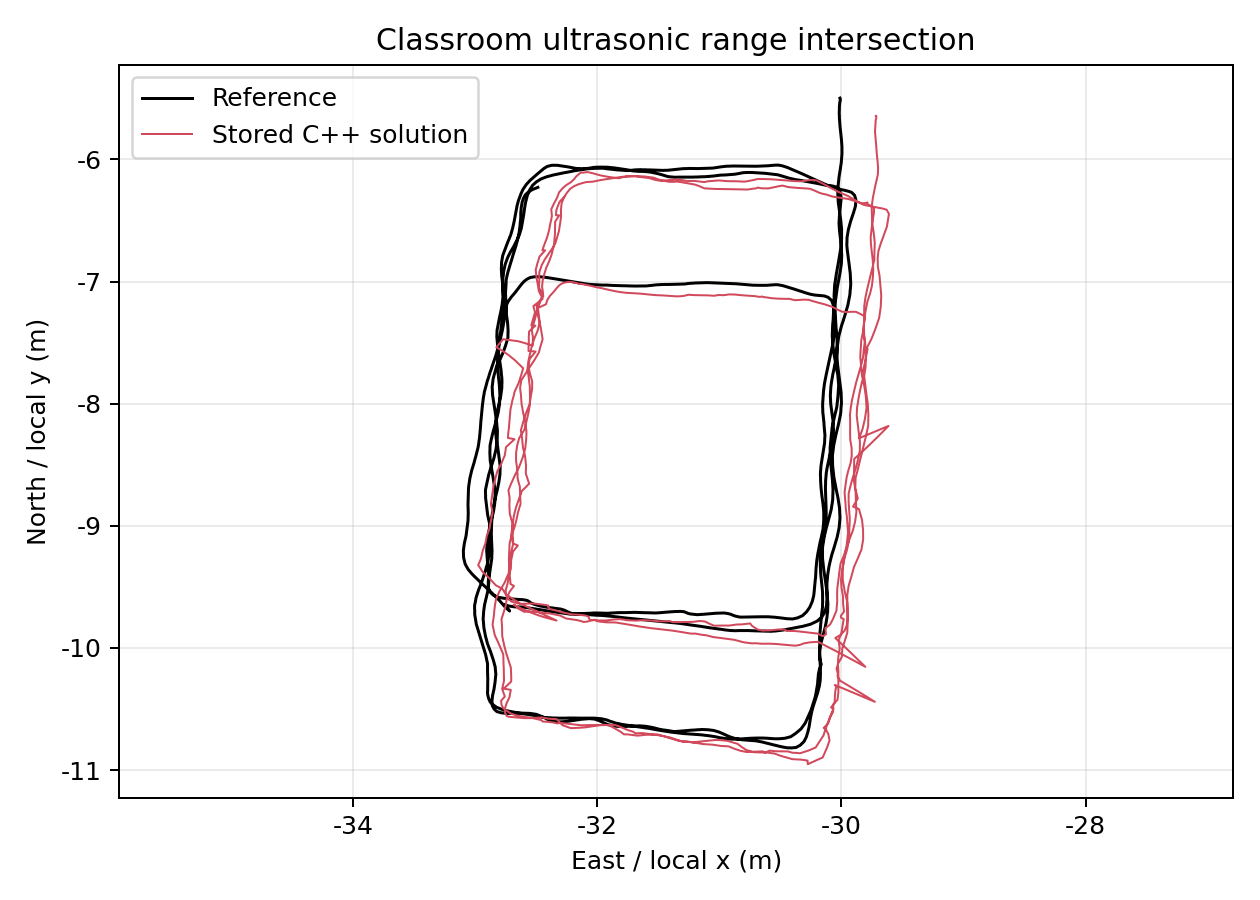
\includegraphics[width=.78\linewidth]{classroom_range_track.png}
\caption{教室超声定位轨迹及时间插值参考轨迹}
\label{fig:classroom}
\end{figure}
图~\ref{fig:classroom-error} 将按时间匹配的水平位置误差与测距拟合 RMS 并列展示。横轴为相对时间，左图纵轴为相对参考轨迹的二维坐标误差，右图纵轴为测距方程残差。两者不是同一误差量：本次位置 RMSE 为 0.239 m，而测距残差中位数仅 0.0099 m；残差较小不保证位置必然准确，因为基站几何构型和参考位置插值误差不会由残差直接反映。误差峰值 0.658 m 应结合时间同步、测距多径和参考采样间隔进一步核查。
\begin{figure}[htbp]
\centering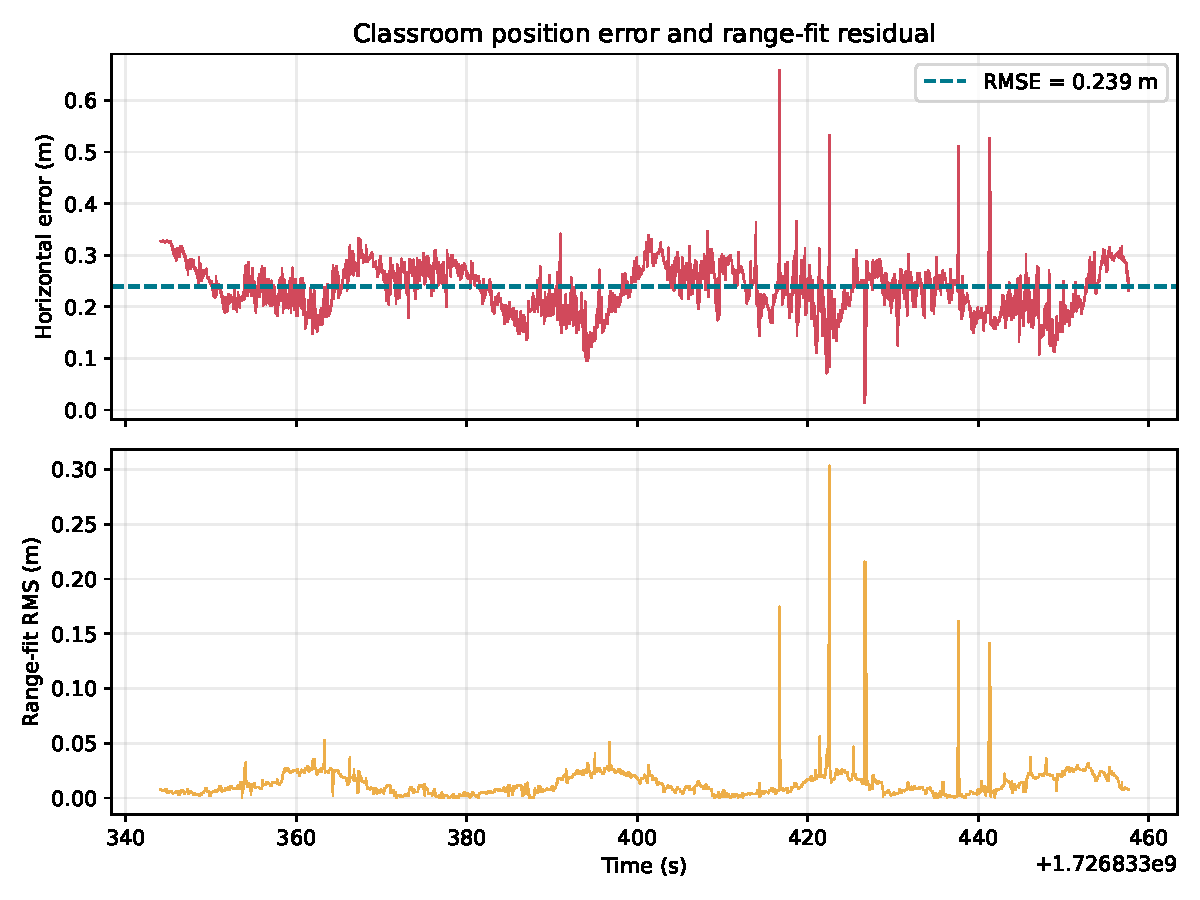
\includegraphics[width=.88\linewidth]{classroom_error_residual.pdf}
\caption{教室超声水平位置误差与测距拟合残差时序}
\label{fig:classroom-error}
\end{figure}
有效解共 7,086 个，按每历元平面误差计算的均值为 0.234 m，RMSE 为 0.239 m，95 分位为 0.304 m，最大值为 0.658 m。测距拟合残差 RMS 的中位数为 0.0099 m。后一个量表示距离方程拟合程度，不能替代位置误差；当基站几何构型不利时，小测距残差仍可能对应较大的位置不确定度。最大位置误差也可能受真值采样插值、基站坐标误差、超声多径/遮挡及时间同步影响。

\subsection{RSS 指纹定位复算}
独立脚本读取 97 个参考点和 1,989 条建库记录，逐 AP 忽略缺失值求均值，再逐个处理 50 个带真值测试时刻。定位函数不接收参考坐标；真值仅在输出位置确定后参与评价。全部 50 个时刻至少存在三个共同有效 AP，故成功率为 100\%。结果轨迹见图~\ref{fig:fingerprint}，误差累计分布见图~\ref{fig:cdf}。

\begin{figure}[htbp]
\centering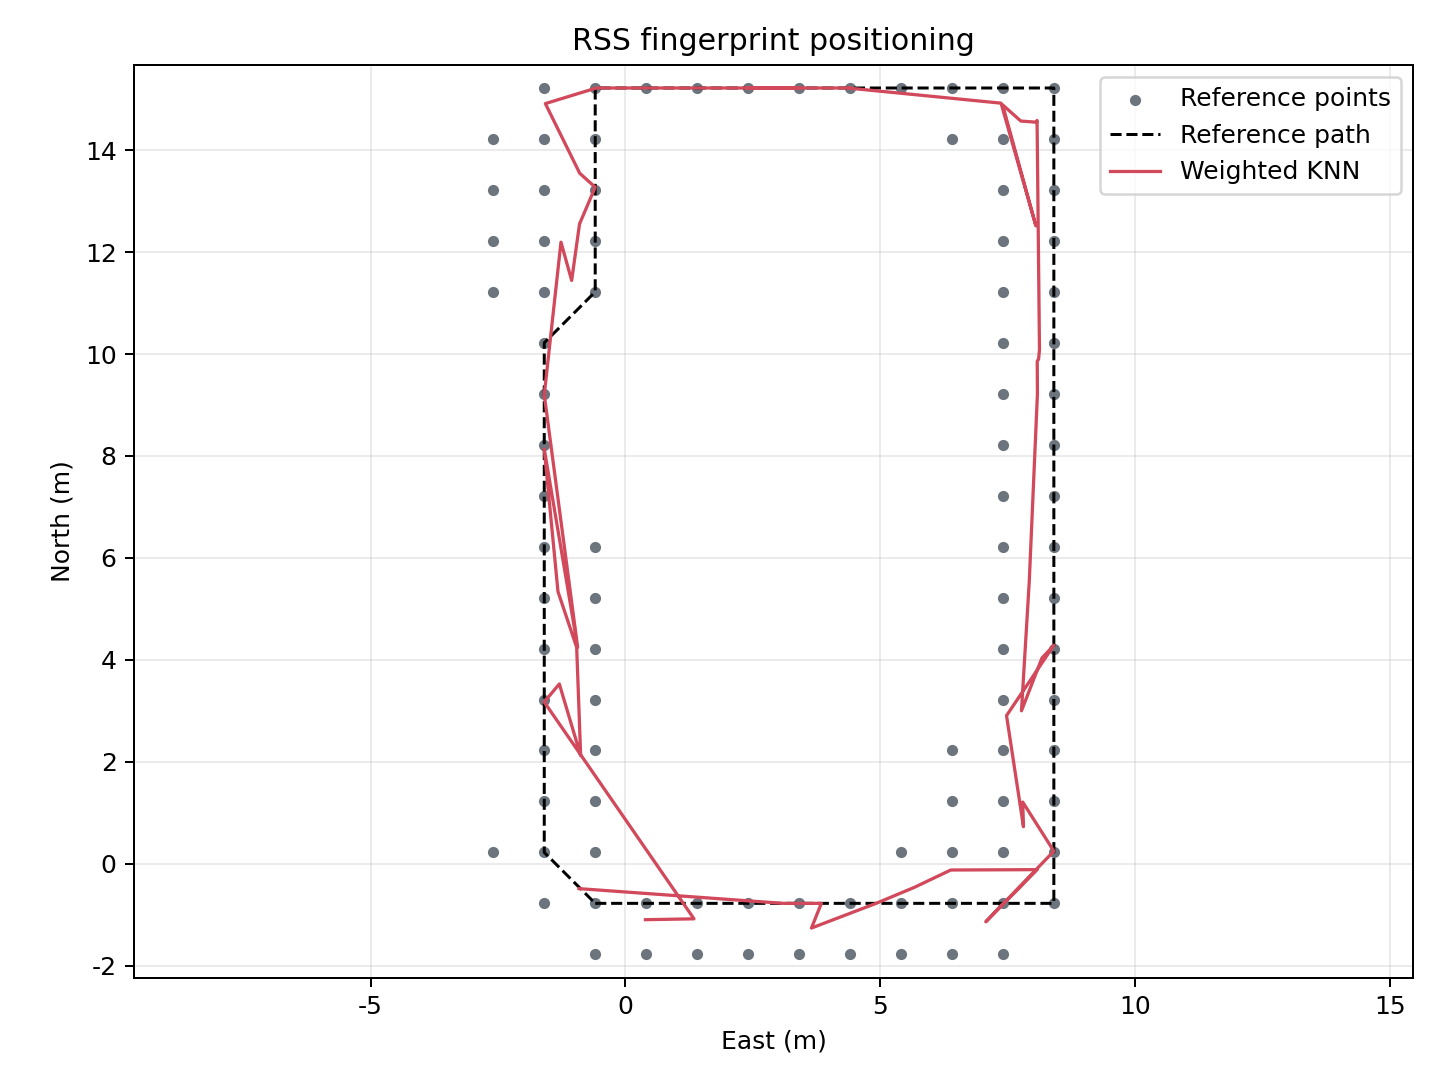
\includegraphics[width=.78\linewidth]{fingerprint_track.png}
\caption{RSS 加权 K 近邻结果与参考轨迹}
\label{fig:fingerprint}
\end{figure}
\begin{figure}[htbp]
\centering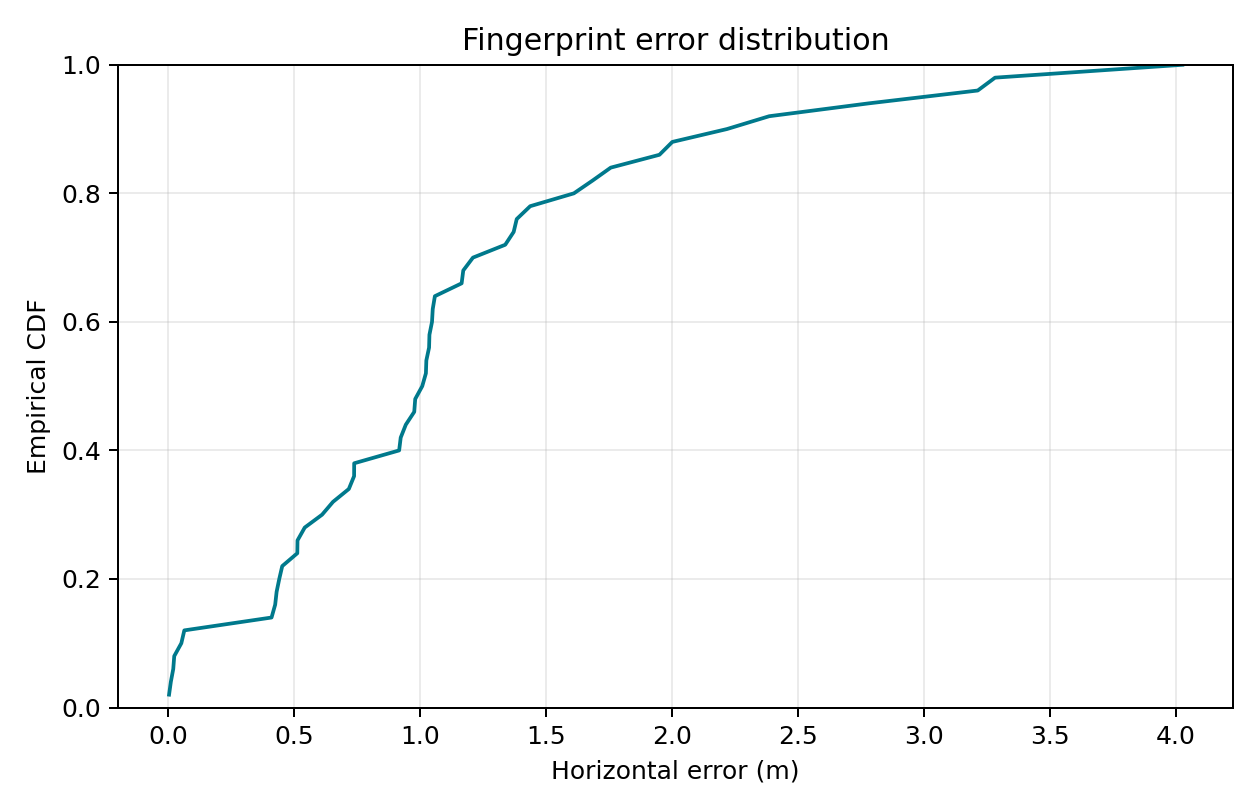
\includegraphics[width=.68\linewidth]{fingerprint_cdf.png}
\caption{指纹水平误差经验累计分布}
\label{fig:cdf}
\end{figure}
\begin{table}[htbp]
\centering\caption{RSS 指纹测试集水平误差统计}\label{tab:finger}
\begin{tabular}{lr}\toprule 指标 & 数值（m）\\\midrule
平均误差 & 1.128\\水平 RMSE & 1.422\\中位数 & 1.016\\95 分位 & 3.020\\最大值 & 4.027\\\bottomrule\end{tabular}
\end{table}
平均误差和 RMSE 的差异显示少数较大误差对平方损失有明显贡献；最大误差约 4 m，说明平均指纹匹配会在 RSS 相似但空间相距较远的位置发生混淆。参考点并非规则完整网格（共 97 点），其空间覆盖不均也使加权坐标插值受采样几何约束。测试路径包含转向段，局部 RSS 的可辨识性和测试采集方向/人体遮挡均可能变化。当前单次测试集规模只有 50 历元，不能据此推断跨设备、跨日期或跨建筑的泛化性能。
为量化邻居数对定位的影响，图~\ref{fig:k-sensitivity} 在完全相同的训练库、距离分数和 50 个测试历元上改变 $K$，误差统计列于表~\ref{tab:k-sensitivity}。$K=1$ 时 RMSE 为 1.311 m，$K=3$ 时为 1.422 m，$K=10$ 时增至 1.725 m；在此小测试集和当前加权规则下，纳入更多邻居会把 RSS 相近但空间位置不同的参考点带入平均，产生位置平滑偏移。该结论只描述本测试集，不能推导出普遍最优的 $K$。
\begin{figure}[htbp]
\centering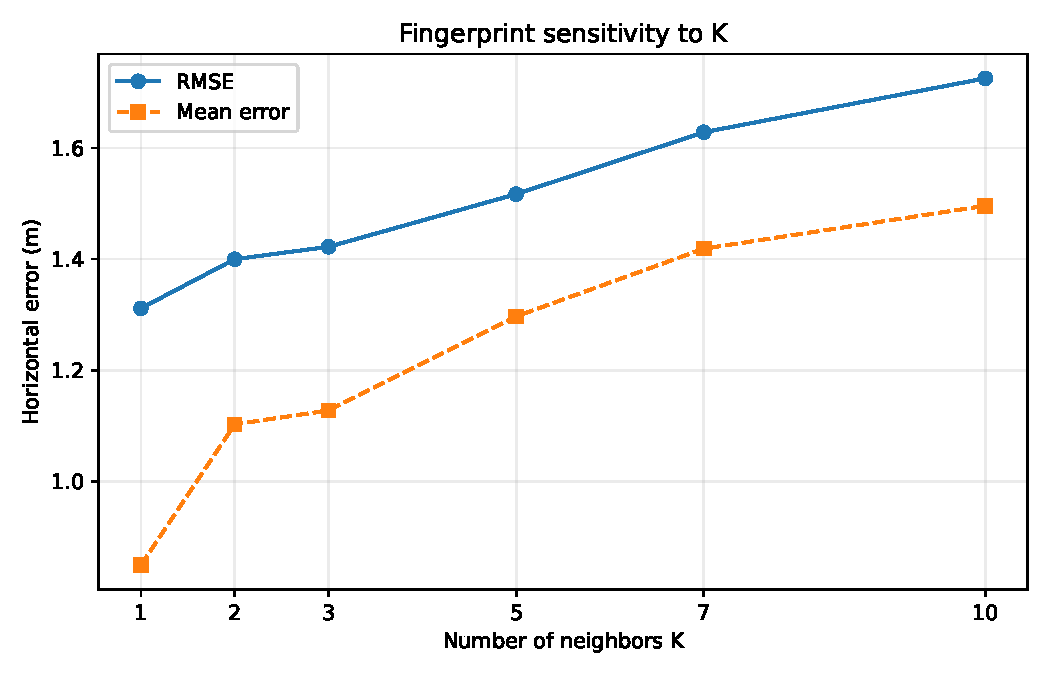
\includegraphics[width=.72\linewidth]{fingerprint_k_sensitivity.pdf}
\caption{指纹加权 KNN 对邻居数 $K$ 的敏感性}
\label{fig:k-sensitivity}
\end{figure}
\begin{table}[htbp]
\centering\caption{不同邻居数下的指纹定位误差}\label{tab:k-sensitivity}
\begin{tabular}{rrrrr}\toprule $K$ & 样本数 & 平均误差（m） & RMSE（m） & 95\%分位（m）\\\midrule
1 & 50 & 0.849 & 1.311 & 3.000\\
2 & 50 & 1.103 & 1.400 & 2.900\\
3 & 50 & 1.128 & 1.422 & 3.020\\
5 & 50 & 1.297 & 1.517 & 2.689\\
7 & 50 & 1.419 & 1.628 & 2.913\\
10 & 50 & 1.496 & 1.725 & 3.280\\\bottomrule\end{tabular}
\end{table}

\subsection{PDR 轨迹与参考位置对照}
本报告没有在原始目录重跑 C++ PDR 主程序，因为它固定写入源码树内的输出目录。为保持原工程只读，采用项目现存的 \texttt{pdr\_result.csv}（6,829 个历元）作为程序输出，对其作独立后处理；参考轨迹由 588 个时间标记的经纬度样本按首点构造局部切平面坐标，并线性插值到步伐时刻。共有 592 个检测步伐，时间覆盖 0 至 341.4 s。该比较包含起始坐标系对准、航向零方向、固定步长模型和参考轨迹插值等共同影响。

\begin{figure}[htbp]
\centering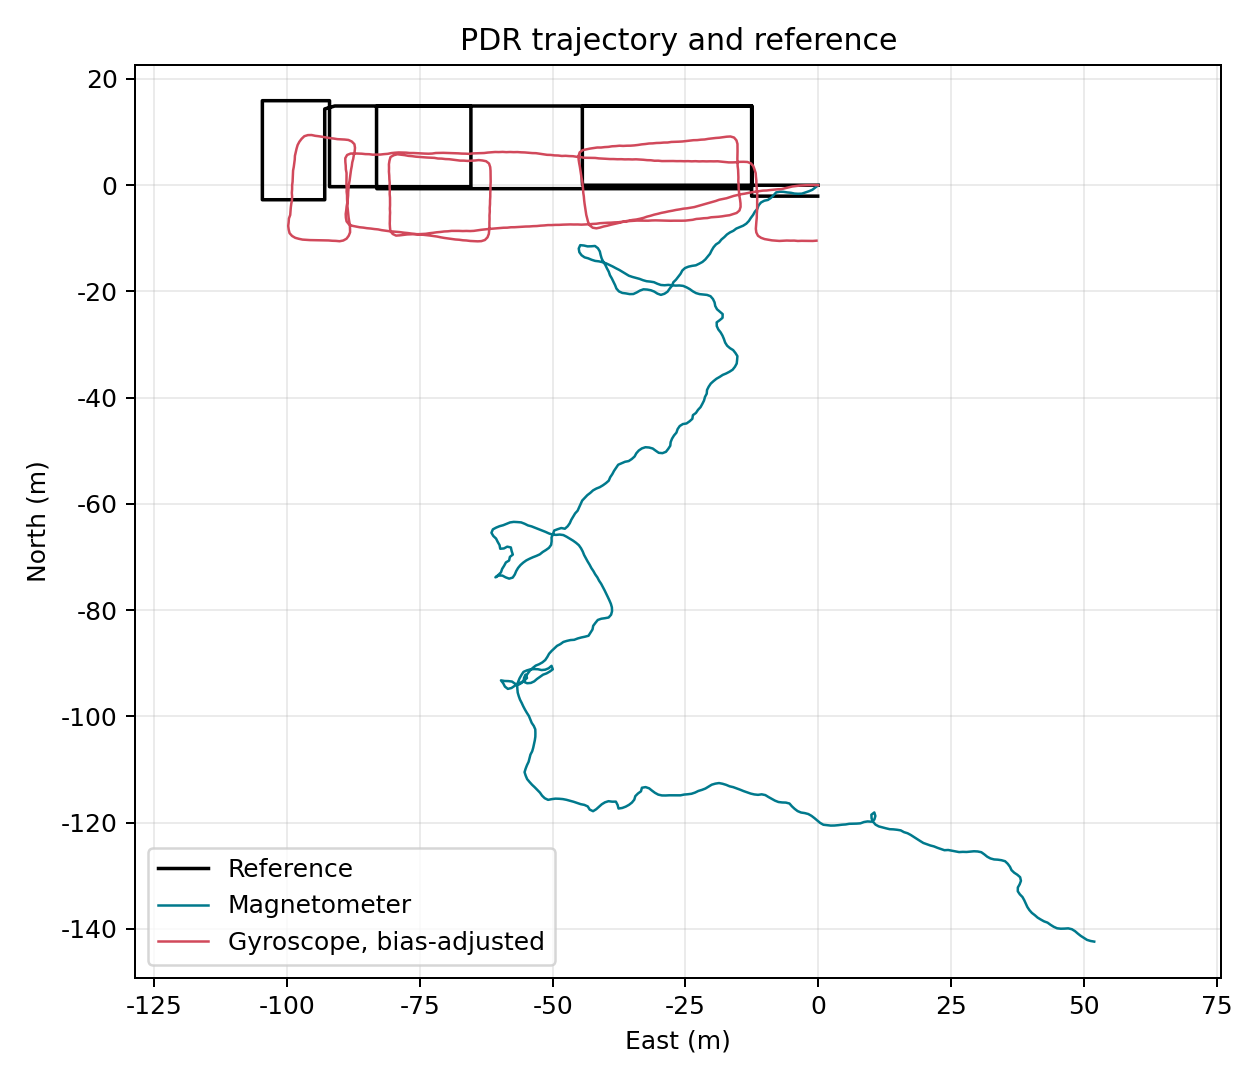
\includegraphics[width=.72\linewidth]{pdr_track.png}
\caption{参考轨迹、磁航向 PDR 与补偿陀螺航向 PDR}
\label{fig:pdr}
\end{figure}
以项目中补偿陀螺轨迹在步伐时刻对参考位置进行比较，误差均值 8.103 m、RMSE 8.381 m、95 分位 10.533 m，末步误差 8.383 m。该误差远大于单步长度，表明仅增加固定的 $0.25^\circ/\mathrm{s}$ 角速度补偿并不足以保证长期轨迹与参考轨迹一致。由于报告使用的是已有 PDR 轨迹输出且没有对起始航向作拟合配准，不能把数值归因于某一项传感器误差；需进一步核查传感器坐标系定义、航向正方向、磁偏角、参考轨迹与采样时钟同步，并对步长和陀螺零偏进行标定。固定步长误差会随步数累积，航向误差则会造成横向漂移。
图~\ref{fig:pdr-raw} 按时间展示程序输出中的三轴加速度、角速度和磁场观测，纵轴分别标出 SI 加速度、弧度每秒角速度及微特斯拉磁场。图~\ref{fig:pdr-signals} 将加速度模及步伐标记、平滑横滚/俯仰和磁/补偿陀螺航向按时间排列。加速度模用于观察步伐检测触发与动态变化；姿态角反映调平后的机体倾斜；航向曲线显示磁方位与陀螺积分在长时间内的差异。所有序列来自项目已保存的 C++ 结果文件，并非原始手机传感器文件重新计算。图~\ref{fig:pdr-error} 给出 592 个检测步时刻的水平误差，横轴为时间、纵轴为与插值参考轨迹的平面距离。误差 RMSE 为 8.381 m，时间变化表明偏差持续存在，因而不能用末点偏差单独描述整段轨迹。
\begin{figure}[htbp]
\centering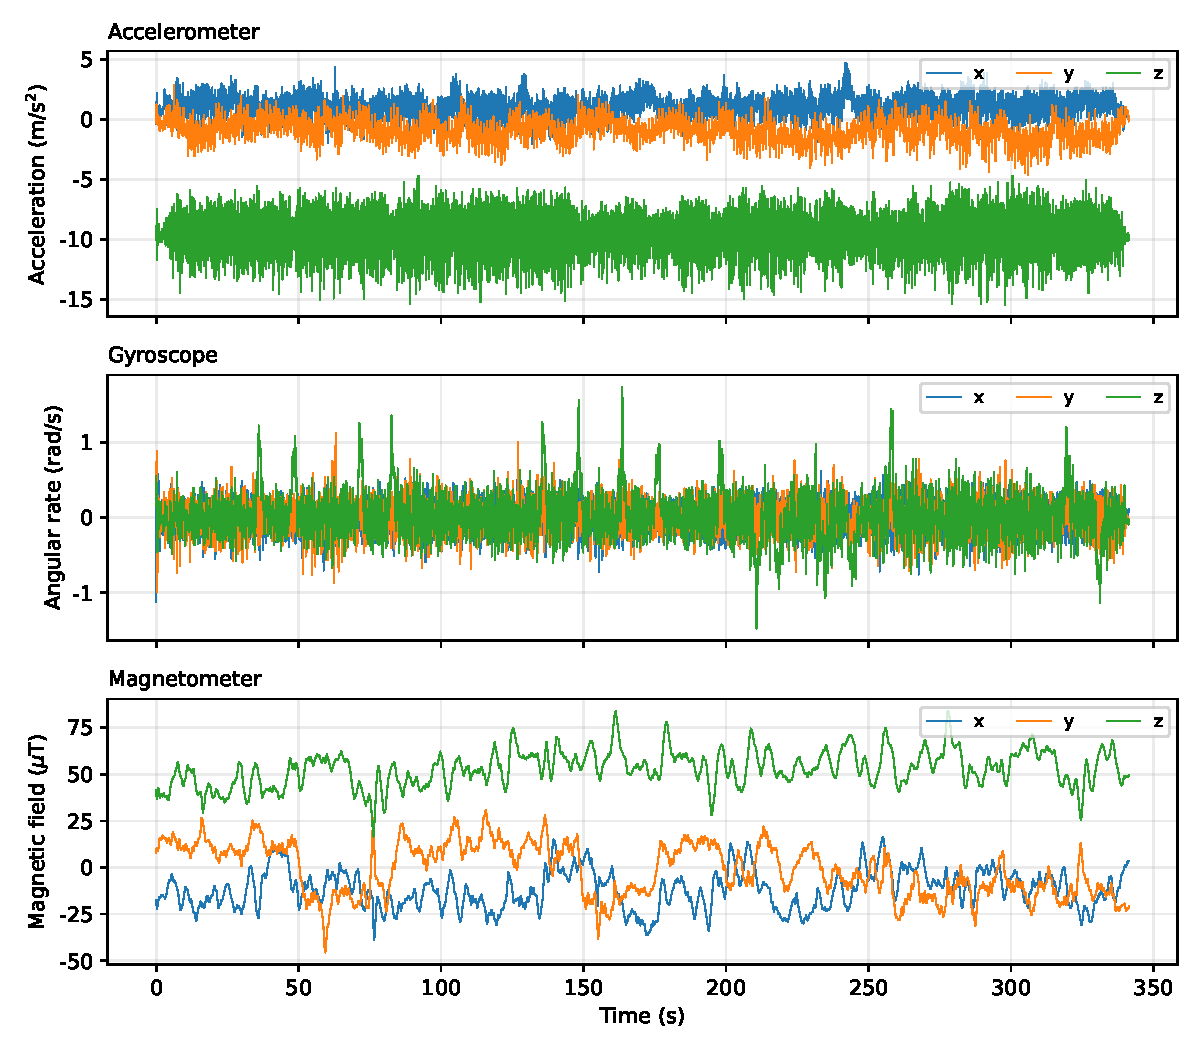
\includegraphics[width=.88\linewidth]{pdr_raw_sensors.pdf}
\caption{PDR 程序记录中的三轴加速度、角速度与磁场观测}
\label{fig:pdr-raw}
\end{figure}
\begin{figure}[htbp]
\centering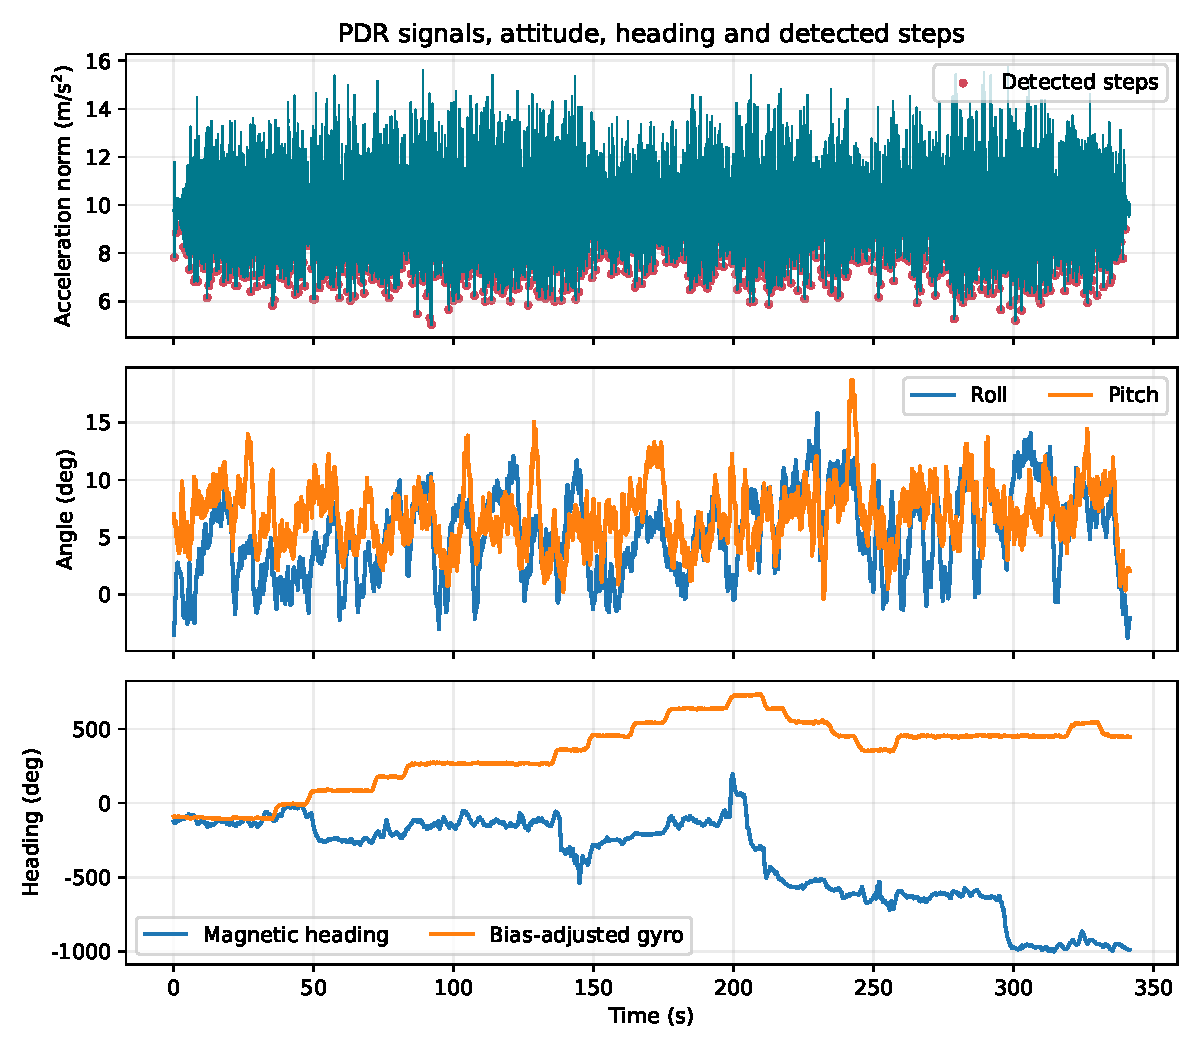
\includegraphics[width=.90\linewidth]{pdr_signals.pdf}
\caption{PDR 加速度模、姿态角、航向与步伐检测时序}
\label{fig:pdr-signals}
\end{figure}
\begin{figure}[htbp]
\centering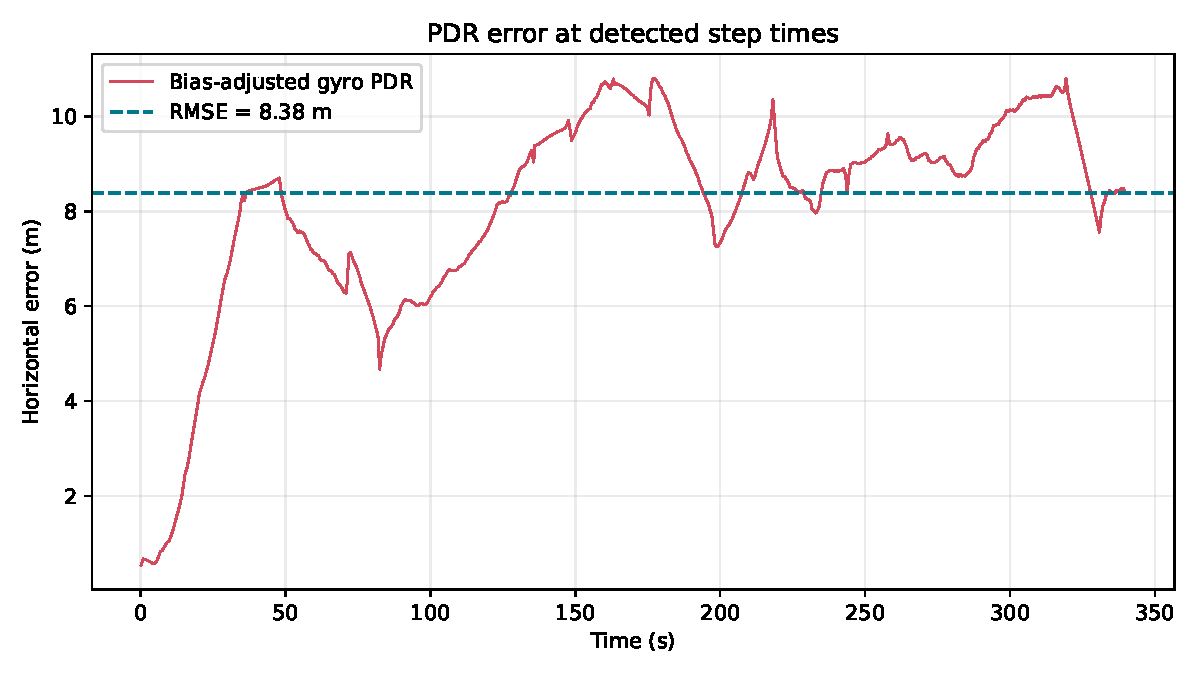
\includegraphics[width=.84\linewidth]{pdr_error_time.pdf}
\caption{PDR 在步伐时刻的水平位置误差}
\label{fig:pdr-error}
\end{figure}

\subsection{UWB 标签二维轨迹与垂向偏差}
实例报告还展示了 UWB 位置轨迹。本项目 tag 2 目录同时提供 C++ 解算结果和真值，可以按时间戳严格匹配而不依赖行序。本次 6,207 条估计中有 5,971 条与 5,971 条真值时间戳相同；仅在该交集上统计水平误差。图~\ref{fig:uwb} 左侧横纵轴为真值/估计的 $x,y$ 坐标（m），右侧横轴为匹配段起点后的秒数，纵轴为水平误差。水平 RMSE 为 0.108 m，均值为 0.084 m，95 分位为 0.189 m。图~\ref{fig:uwb-z} 的上图比较真值高度与估计高度，下图表示逐历元高度误差及其平均偏差。高度平均偏差为 $-0.821$ m，垂向 RMSE 为 0.845 m，说明此组结果适合评价平面轨迹，但三维误差受明显高度系统差影响。当前未找到可核验的 DOP 时序输出，故不仿造实例报告中的 DOP 曲线；UWB 结果文件也属于项目已存 C++ 输出的后处理，不宣称本轮重新运行了 UWB 主程序。
\begin{figure}[htbp]
\centering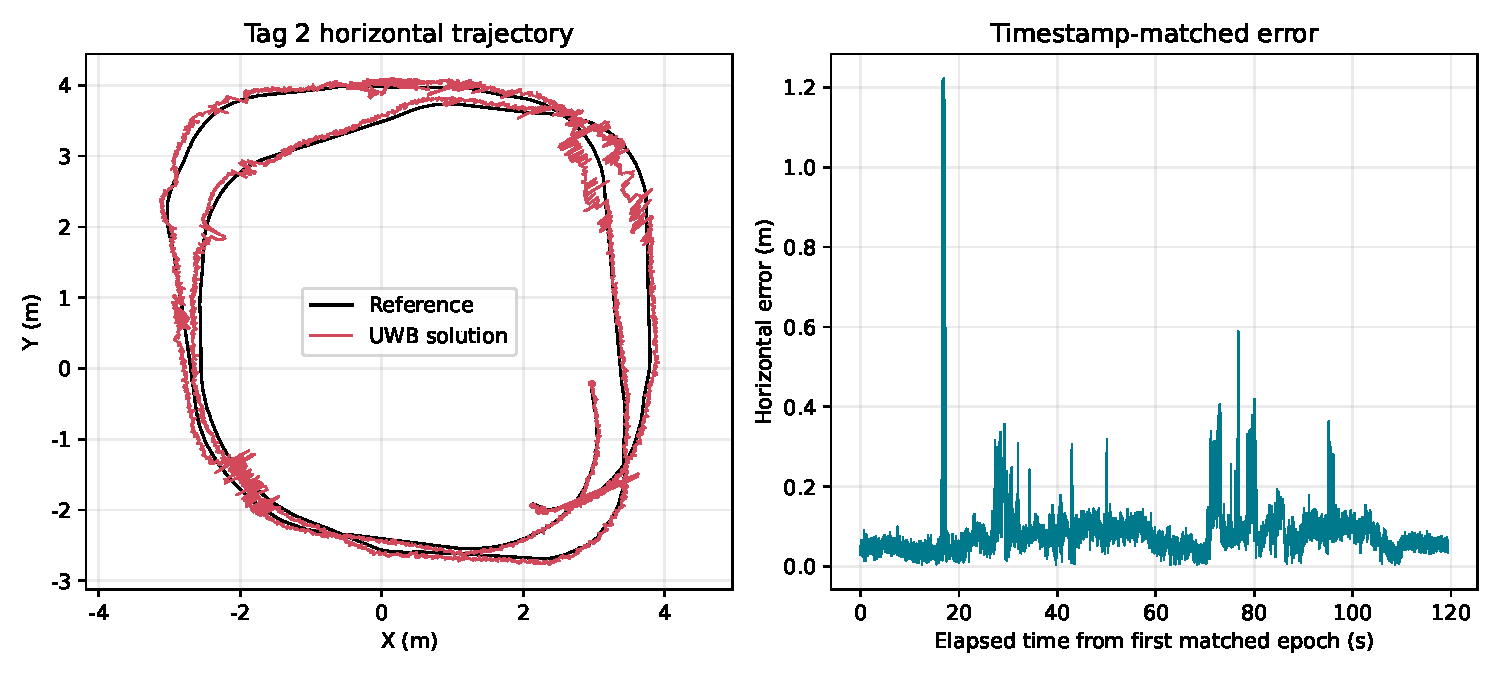
\includegraphics[width=.96\linewidth]{uwb_tag2_track_error.pdf}
\caption{UWB tag 2 平面轨迹及时间戳匹配的水平误差}
\label{fig:uwb}
\end{figure}
\begin{figure}[htbp]
\centering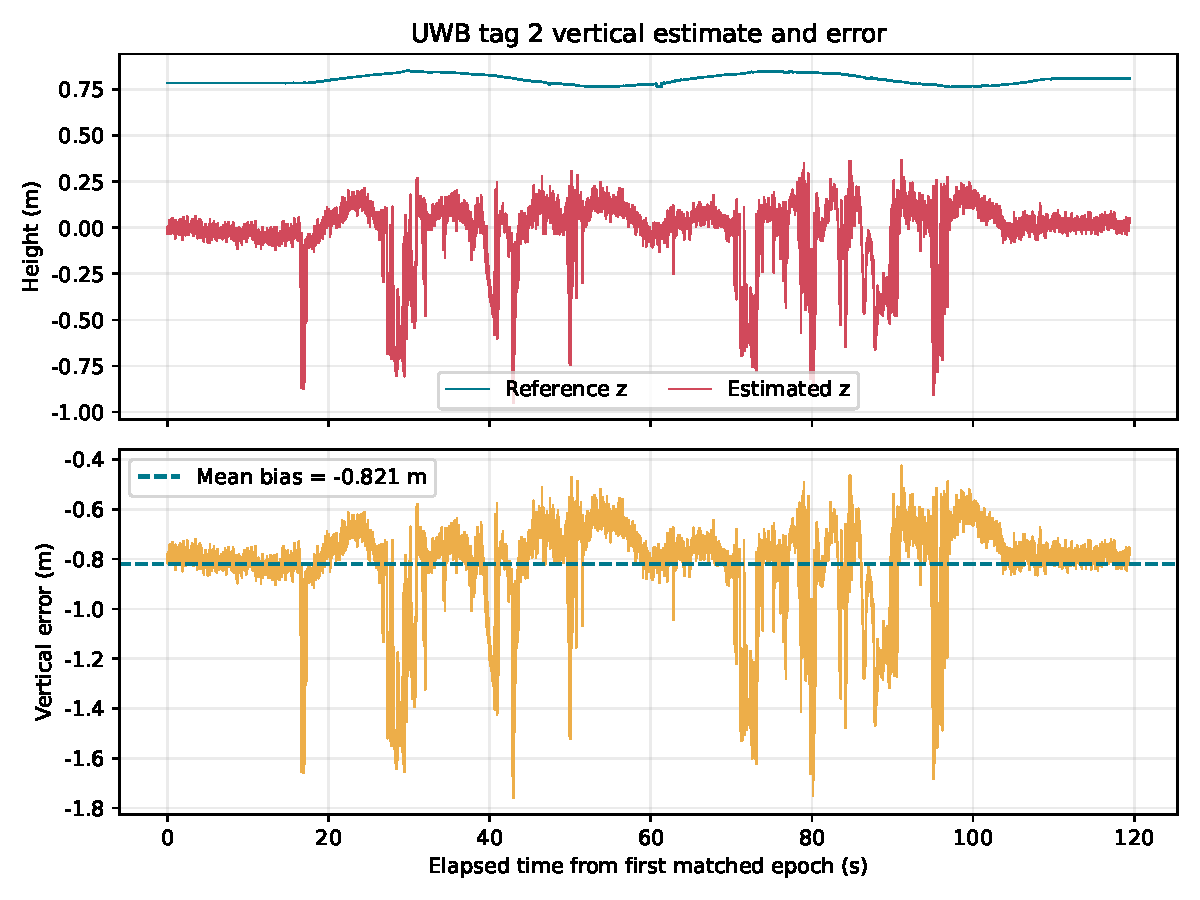
\includegraphics[width=.84\linewidth]{uwb_tag2_vertical_error.pdf}
\caption{UWB tag 2 真值/估计高度及垂向误差}
\label{fig:uwb-z}
\end{figure}

\section{方法比较与讨论}
\begin{table}[htbp]
\centering\caption{三种方法的观测、误差特征与本次证据等级}\label{tab:compare}
\begin{tabular}{p{2.5cm}p{3.2cm}p{4.0cm}p{3.1cm}}
\toprule 方法 & 主要观测 & 主要误差/优势 & 本次结果证据 \\
\midrule 几何距离交会 & 到已知基站的距离 & 几何条件直接影响解算精度；可解释、定位精度高，但要求基础设施和可靠测距 & 对已有教室 C++ 输出重算真值误差 \\
RSS 指纹 & 多 AP 的接收功率向量 & 部署简单、无需测距模型；依赖场景稳定、建库密度与设备一致性 & 从原始训练/测试数据重新计算 \\
PDR & 加速度、角速度、磁场 & 自主连续但位置漂移积累；步长、步检和航向均需标定 & 对项目已有 C++ 结果作真值对齐复核 \\
\bottomrule
\end{tabular}
\end{table}
三种方法的误差指标来自不同场地、不同参考条件，不宜将表~\ref{tab:finger} 与教室误差简单解释为算法优劣排序。距离交会报告的是独立真实参考轨迹下的二维误差；指纹报告的是另一个场地中 50 个离散历元的水平误差；PDR 对齐受到参考轨迹与设备坐标方向的影响。它们说明各方法各自的数据条件下的行为，而非严格控制变量对比。

Android 采集软件说明了手机端数据采集、点号关联和按会话保存的流程，配套 MATLAB 脚本负责传感器、Wi-Fi 与 GPS 数据转换。课程项目 Python 脚本还可对指定会话绘制传感器时序和 Wi-Fi 热点分布。但 Android 示例采集会话与指纹/PDR实验文件不是同一数据集，因此不能把该采集样例的统计混入定位结论。
为展示采集记录实际可用性，图~\ref{fig:android-sensors} 统计会话时间范围内的陀螺仪和加速度三轴样本；文件中分别有 6,841 和 6,782 条记录。图~\ref{fig:android-wifi} 按相对时间汇总 Wi-Fi 扫描记录数，328 次扫描共包含 379 个不同 BSSID，平均每次扫描约 88.4 条 AP 记录；图~\ref{fig:android-rss} 展示按出现扫描次数排序的四个 BSSID 的 RSS 时序，横轴是会话相对秒数，纵轴为接收功率 dBm。不同热点随时间呈现不同幅度的波动，反映接入点可见性和无线信道变化；因文件没有可确认的参考坐标，不将这些 RSS 曲线解释为距离模型或定位误差。数据用于说明传感器与无线观测的采样特征，不与其他采集会话的定位结果混合。
\begin{figure}[htbp]
\centering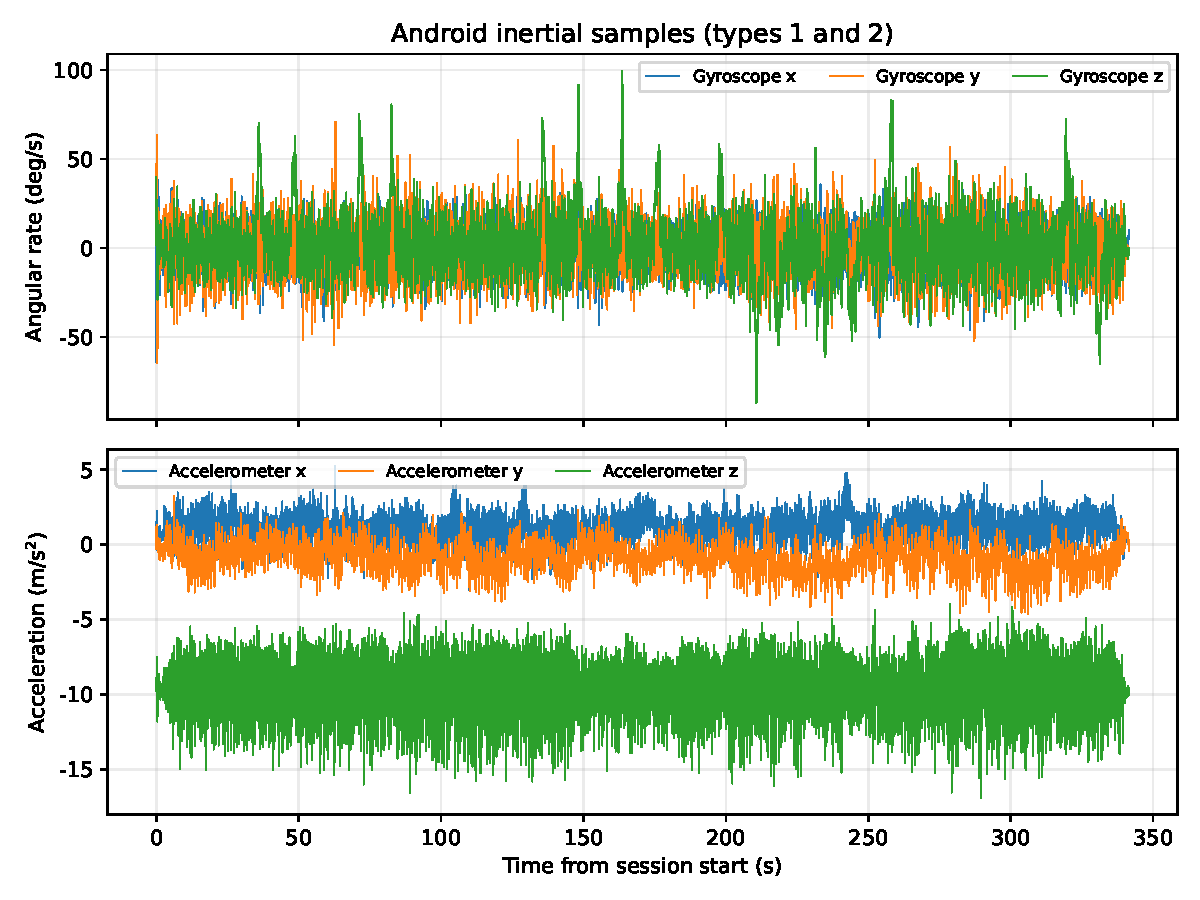
\includegraphics[width=.88\linewidth]{android_inertial_timeseries.pdf}
\caption{Android 样例会话中的陀螺仪与加速度计三轴观测}
\label{fig:android-sensors}
\end{figure}
\begin{figure}[htbp]
\centering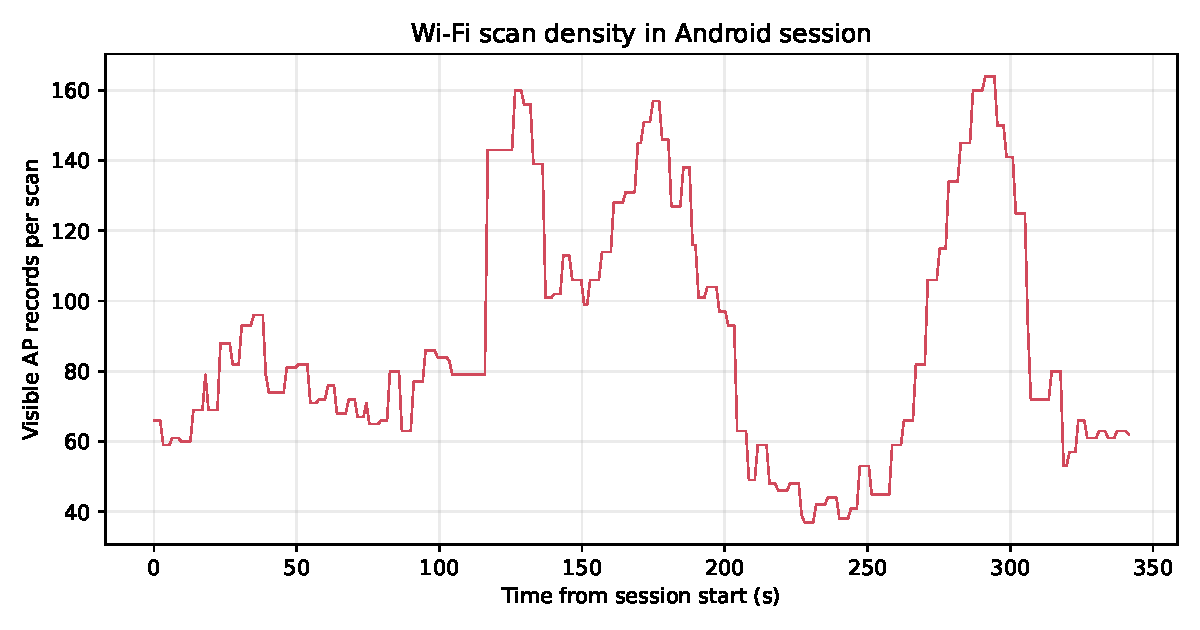
\includegraphics[width=.84\linewidth]{android_wifi_scan_density.pdf}
\caption{Android 样例会话的 Wi-Fi 扫描记录数时序}
\label{fig:android-wifi}
\end{figure}
\begin{figure}[htbp]
\centering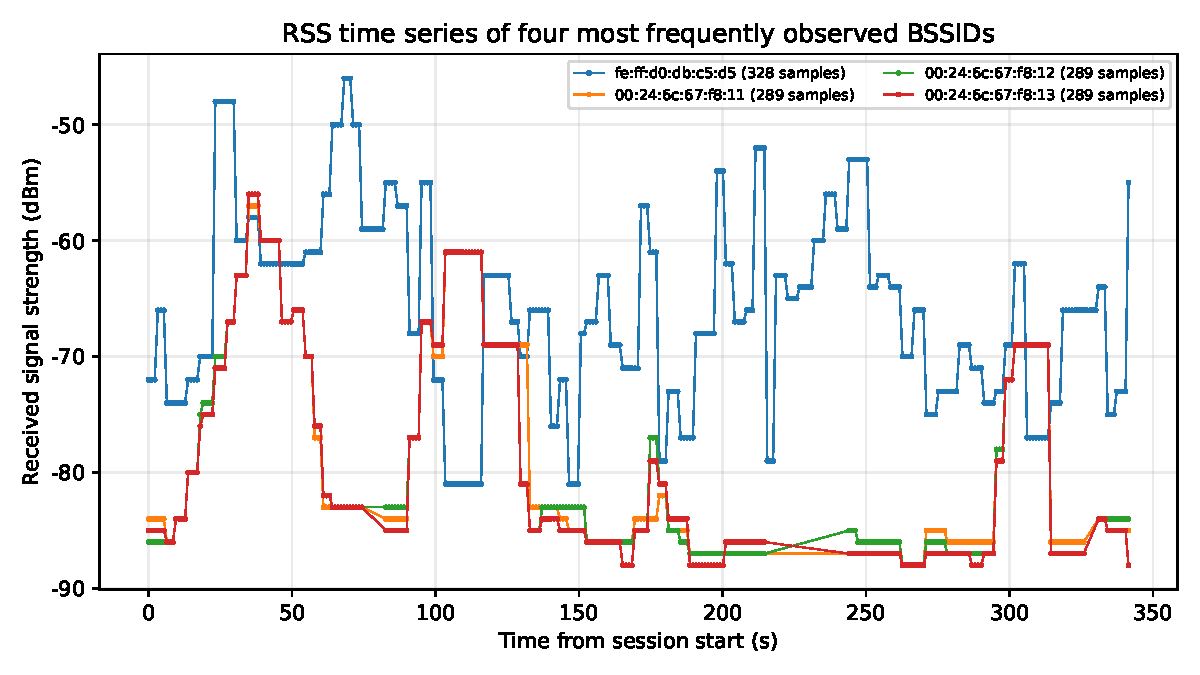
\includegraphics[width=.84\linewidth]{android_wifi_rss_timeseries.pdf}
\caption{Android 样例中出现频次最高的四个 BSSID 的 RSS 时序}
\label{fig:android-rss}
\end{figure}
